\chapter{Management Summary  -- SUBJECT TO CHANGE --}

\section{Ausgangslage}
Der Internetbrowser ist heute mehr denn je das Zuhause für immer komplexer werdende Applikationen. Durch die Leistungssteigerung und immer ausgefeilteren Möglichkeiten nutzen ihn heutzutage nicht mehr nur Unternehmen als Schnittstelle zwischen Angestellten und Anwendungen. So wäre der Google Mail Client oder auch Facebook, um nur zwei prominente Beispiele zu nennen, in ihrer aktuellen, interaktiven Form ohne die grossen Fortschritte im Bereich Browsertechnologie der letzten Jahre nicht umsetzbar.

Erwartungsgemäss können traditionelle Paradigmen und Softwarearchitekturkonzepte mit der neuen Technologie nicht mehr immer Schritt halten und Lösungen für wiederkehrende Probleme bieten. Diese Bachelorarbeit soll neue Trends auf dem Gebiet der Webapplikationen kritisch analysieren und gleichzeitig zukunftsweisende Inputs für das Unterrichtsmodul ``Internettechnologien'' liefern.

\section{Vorgehen}
In einer Vorstudie wurden zunächst drei grundlegende Fragen geklärt: Welche der insgesamt 28 Softwarearchitekturkonzepte aus der Aufgabenstellung sollen bearbeitet werden? Welche Applikation kann die ausgewählten Konzepte optimal veranschaulichen? Und mit welcher Technologie sollen die ausgewählten Konzepte demonstriert werden?

Nach der ausführlichen Evaluation des Konzeptkatalogs und der Auswahl von 22 Konzepten entschied sich das Projektteam eine vergleichsweise simple Aufgabenverwaltung für Wohngemeinschaften mit dem Namen ``Roomies'' umzusetzen. Damit wird sichergestellt, dass der Fokus auf die Demonstration der Architekturkonzepte gelegt werden kann. Als wichtigen Schritt Richtung ``Bleeding Edge'' wurde zudem entschieden, sowohl server- als auch clientseitig auf JavaScript zu setzen.

\section{Ergebnisse}
\begin{figure}[H]
	\centering
	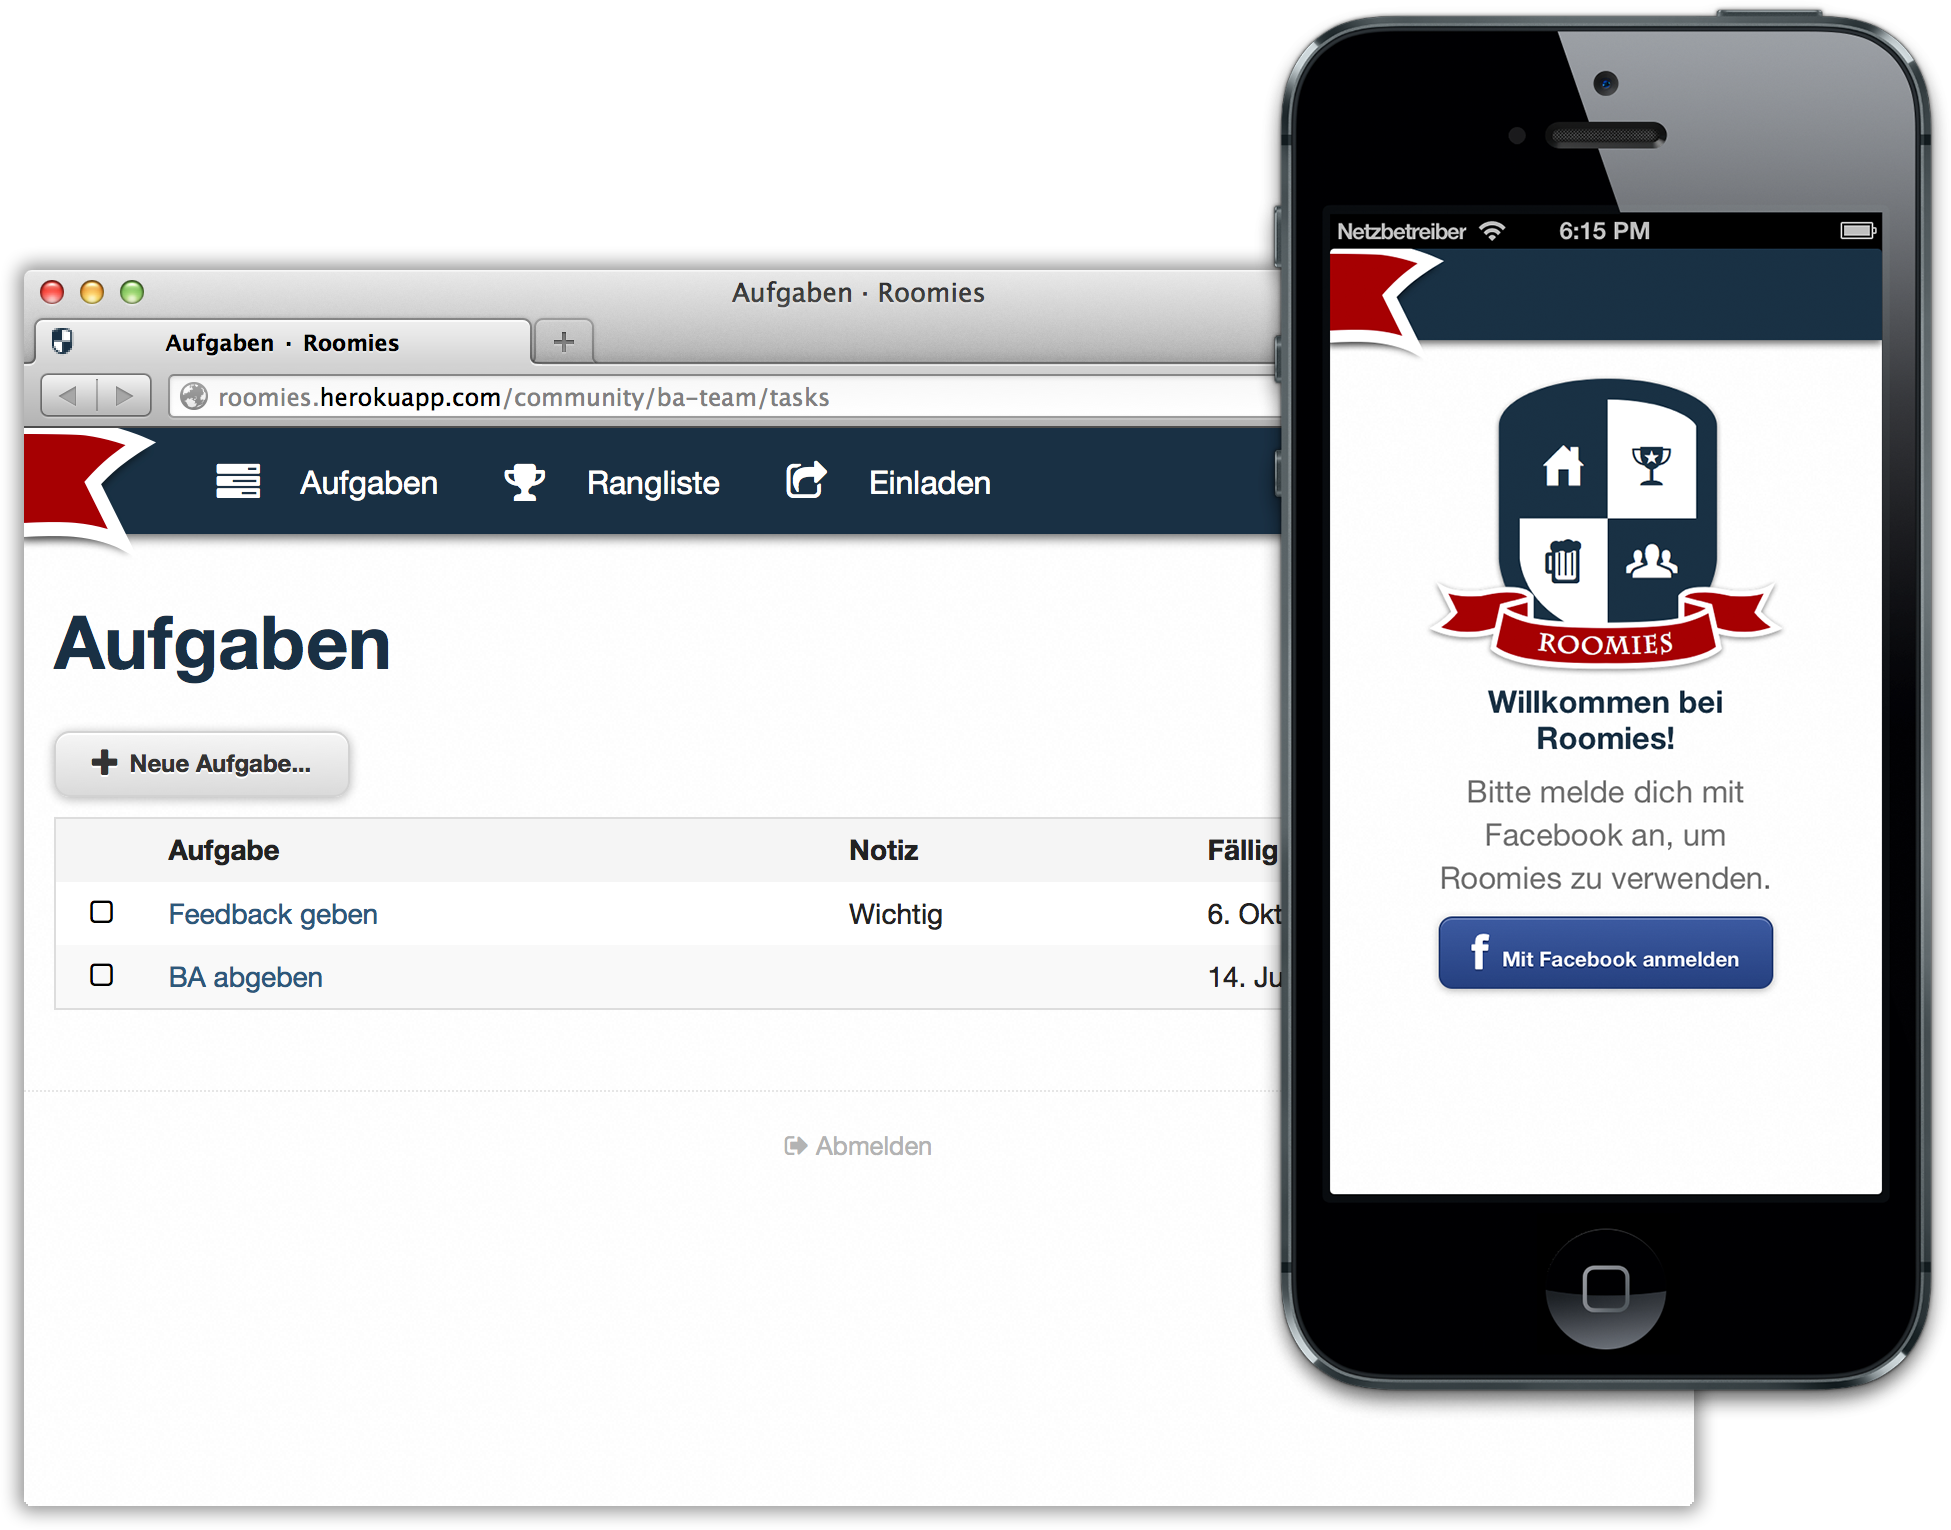
\includegraphics[width=12cm]{content/images/roomies-ui.png}
	\caption{Aufgabenverwaltung \emph{Roomies} zur Konzeptdemonstration}
\end{figure}

Die Studie am Ende dieser Bachelorarbeit bietet einen tiefen Einblick in die Entwicklung einer verteilten, JavaScript-basierten Client-Server-Webapplikation. Die ausführlichen Analysen und persönlichen Stellungnahmen des gesamten Projektteams bewerten die untersuchten Softwarearchitekturkonzepte kritisch. Ergänzend dazu bietet der Quellcode von ``Roomies'' anschauliche Beispiele zu jedem der 22 Konzepte. Besondere Aufmerksamkeit wurde dabei dem Konzept ``Unobtrusive JavaScript'' zuteil. Basierend auf ``Backbone.js'' wurde eine eigene quelloffene Bibliothek namens ``barefoot'' entwickelt, welche ohne grösseren Mehraufwand den gleichen Quelltext sowohl im Browser des Endbenutzers als auch auf der Serverkomponente lauffähig macht.

\section{Ausblick}